\documentclass{article}
\usepackage{arrayjob}
\usepackage[spanish, es-tabla]{babel}
\usepackage{booktabs}
\usepackage{caption}
\usepackage{csvsimple}
\usepackage{fancyhdr}
\usepackage{float}
\usepackage{fontspec}
\usepackage[footskip=5pt, textheight=530pt]{geometry}
\usepackage{graphicx}
\usepackage{hyperref}
\usepackage[utf8]{inputenc}
\usepackage{multirow}
\usepackage{python}
\usepackage{titling}
\usepackage{xcolor}

\setmainfont [ 
 Path = fonts/ , 
 UprightFont = *Regular ,
 BoldFont = *Bold ,
 ItalicFont = *Italic ,
 Extension = .otf
]{CronosPro}

\pagestyle{fancy}

%%%%% cosas del titulo %%%%
\newcommand{\HRule}{\rule{\linewidth}{0.5mm}}


\DeclareUrlCommand{\url}{%
    \def\UrlFont{\color{blue}\normalfont}%      Adding a little color 
    \def\UrlLeft##1\UrlRight{\underline{##1}}%  Underlining the url
    }
%%%%%%%%%%%%%%%%%%%%%%%%%%%

%\lhead{
\includegraphics[width=2cm]{./logos/conabio.png}}
%\chead{
\includegraphics[width=2cm]{./logos/semarnat.png}}
%\rhead{
\includegraphics[width=2cm]{./logos/conanp.png}}
%\rhead{
\includegraphics[width=2cm]{./conabioLogo.jpg}}
%\lfoot{
\includegraphics[width=2cm]{./logos/gefResiliencia.png}}
\lfoot{\vspace{5mm} \HRule \\ \small{Comisi\'on Nacional para el Conocimiento y Uso de la Biodiversidad \\
Liga Perif\'erico-Insurgentes Sur 49031 \\
Parques Del Pedregal, Del. Tlalpan, \\
Ciudad de M\'exico, C.P. 14010 \\
\url{www.gob.mx/conabio} \\
\url{www.biodiversidad.gob.mx/pais/cambio_climatico.html} }}
%Ciudad de M\'exico, C.P. 14010 \\
%www.gob.mx/conabio \\
%www.biodiversidad.gob.mx/pais/cambio_climatico.html}
%\rfoot{
\includegraphics[width=2cm]{./logos/pnudUnamBiol.png}}
%\cfoot{http://www.conabio.gob.mx}

%\usepackage{pgfplotstable}


%\newcommand{\test}{\input{id.txt}\unskip}
%\graphicspath{{/var/www/html/nrb/Mapps/Conabio/reportesPDF/LaTeX/341810900dir/}}
%\graphicspath{{./LaTeX/341810900dir/}}
%\graphicspath{{/var/www/html/nrb/Mapps/Conabio/reportesPDF/LaTeX/341810900dir/}}

\definecolor{red}{RGB}{153, 8, 22}
\definecolor{yellow}{RGB}{227, 191, 79}
\definecolor{blue}{RGB}{0, 113, 188}
\definecolor{red2}{RGB}{173, 57, 68}
\definecolor{brown}{RGB}{193, 153, 121}
\definecolor{orange}{RGB}{193, 109, 68}
\definecolor{grey}{RGB}{128, 128, 128}





\begin{document}


	\begin{titlepage}
%\begin{center}
\begin{center}
% 	%\textsc{\Large Spatiotemporal modeling of fuelwood environmental impacts: towards improved accounting for non-renewable biomass}\\[0.5cm]
% 	\textsc{\Large Explorador de cambio clim\'atico y Biodiversidad}\\[0.5cm]

% 	%\textsc{\Large Mofuss: Modeling fuelwood savings scenarios - version 1.0}\\[0.25cm]
% 	\textsc{\Large Comisi\'on Nacional para el Conocimiento y Uso de la Biodiversidad (CONABIO)}\\[0.25cm]


% \HRule \\[0.25cm]
% 	{\huge\textbf{Reporte de areas seleccionadas \\}}
% \HRule \\[0.25cm]
	
% 	\emph{{\large Este es un reporte generado autom\'aticamente que resume la consulta realizada en el explorador de cambio clim\'atico y biodiversidad. \\}}

% 	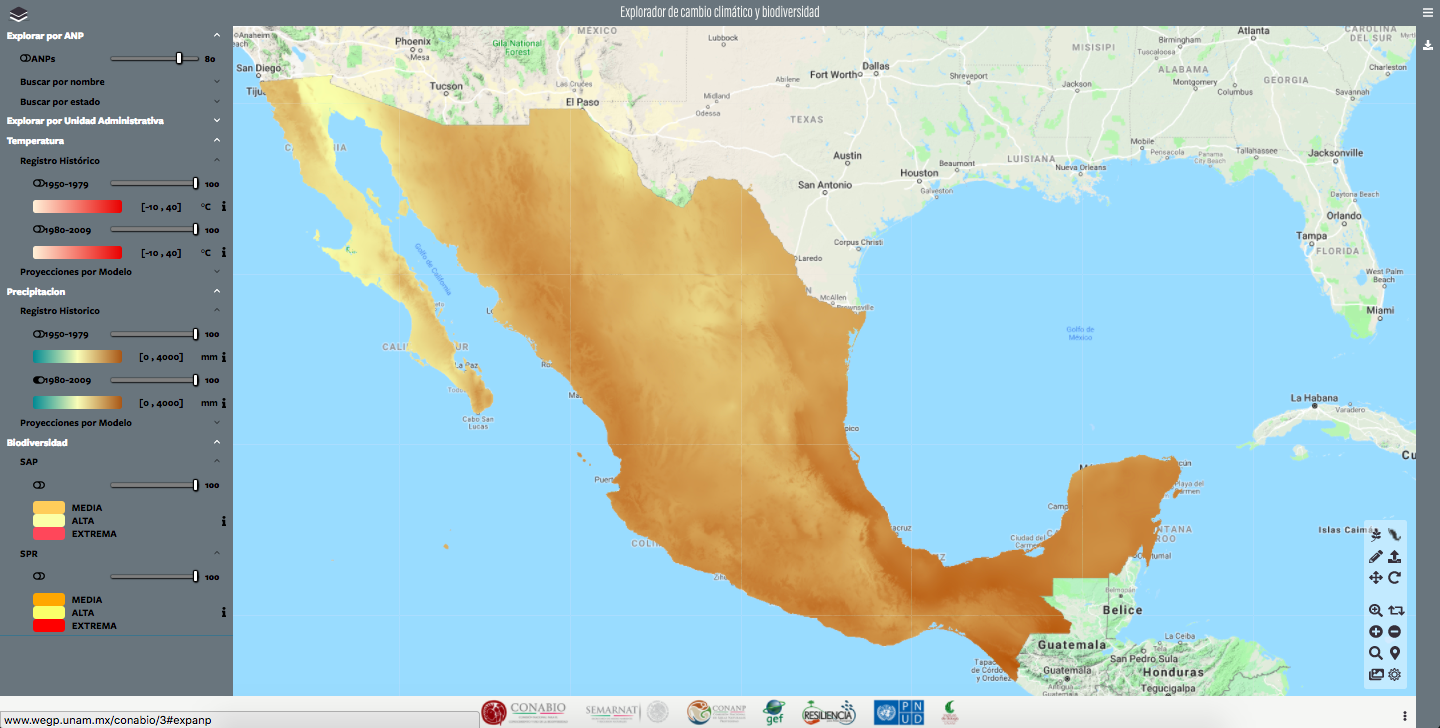
\includegraphics[width=0.9\linewidth]{./logos/entry.png} \\

% 	\textbf{Proyecto financiado por: } \\

	\begin{table}[h!]
	\centering
		%\begin{center}
			\begin{tabular}{ccccc}

				%\multicolumn{3}{c}{
\includegraphics[width=6cm]{./logos/conabio.png}} \\ 
				%
\includegraphics[width=4cm]{./logos/semarnat.png} &
				%
\includegraphics[width=4cm]{./logos/conanp.png} &
				%
\includegraphics[height=2.5cm]{./logos/gef.png} \\

				%
\includegraphics[width=4cm]{./logos/resiliencia.png} &
				%
\includegraphics[width=4cm]{./logos/pnud.png} &
				%
\includegraphics[height=2.5cm]{./logos/unam.png}


				
\includegraphics[width=3cm]{./logos/conabio.png} &
				
\includegraphics[height=2.5cm]{./logos/unam.png} &
				
\includegraphics[width=3cm]{./logos/semarnat.png} &
				
\includegraphics[width=3cm]{./logos/conanp.png} &
				
\includegraphics[width=3cm]{./logos/logoINECC.png} \\

				%\multicolumn{2}{c}{
\includegraphics[height=2.5cm]{./logos/gef.png}} &
				%\multicolumn{2}{c}{
\includegraphics[width=3cm]{./logos/resiliencia.png}} &
				%
\includegraphics[width=3cm]{./logos/pnud.png}

				\multicolumn{2}{c}{
\includegraphics[height=2.5cm]{./logos/gef.png}} &
				\multicolumn{1}{c}{
\includegraphics[width=3cm]{./logos/resiliencia.png}} &
				\multicolumn{2}{c}{
\includegraphics[width=3cm]{./logos/pnud.png}}


			\end{tabular}
		%\begin{center}
	\end{table}
	%\bigskip
	%\bigskip
	\vspace{2.5cm}
	\huge{\textbf{EXPLORADOR DE CAMBIO CLIM\'ATICO Y BIODIVERSIDAD }}\\
	%\bigskip
	\large{COMISI\'ON NACIONAL PARA EL CONOCIMIENTO Y USO DE LA BIODIVERSIDAD \\
	(CONABIO)} \\

	\vspace{2.5cm}

	\textbf{Reporte de la consulta de \'areas inter\'es'} \\
	Reporte generado autom\'aticamente que resume datos de la consulta realizada en
	el \emph{Explorador de cambio clim\'atico y biodiversidad}.
	%\bigskip
	%\bigskip
	%\bigskip
	\vspace{2cm}
	%\small{Conabio, IB-UNAM, Conanp, PNUD, INECC, Reporte de \'areas seleccionadas. Explorador de cambio clim\'atico y biodiversidad. Comisi\'on Nacional para el Conocimiento y Uso de la Biodiversidad, en \ref{http://www.biodiversidad.gob.mx/pais/cambio_climatico.html} Fecha de consulta: }
	%\pagebreak

\end{center}

% \HRule \\[0.25cm]
% { 
% 	\huge \bfseries Summary Report for %\input{../LULCC/TempTables/Country.txt}}
% }
% \HRule \\[0.25cm]
% {
% 	\emph{\large This is an automated report generated by The present document summarizes main results of the model for the red polygon in the map shown here below.\\ } 
% }


% %\includegraphics[width=0.9\linewidth]{../OutBaU/png/Area_of_Interest}

% \textbf{Project funded by:}\\
% %\includegraphics[width=0.2\linewidth]{../LULCC/Wizard_imgs/GACC}
% \end{center}


% \pagebreak 
% %\setlength{\parindent}{0cm}

% \begin{flushleft}

% %A. Ghilardi, R. Bailis, J-F. Mas, R. Drigo, O. Masera. \textbf{Summary Report for \input{../LULCC/TempTables/Country.txt}}- Spatiotemporal modeling of fuelwood environmental impacts. \the\year. CIGA-UNAM and SEI-US. \pageref{lastpage} p.
% \bigskip

\begin{flushleft}
\small{Conabio, IB-UNAM, Conanp, PNUD, INECC, Reporte de \'areas seleccionadas. Explorador de cambio clim\'atico y biodiversidad. Comisi\'on Nacional para el Conocimiento y Uso de la Biodiversidad, en \url{http://www.biodiversidad.gob.mx/pais/cambio_climatico.html} Fecha de consulta: \input{fecha.txt}}
% Comisi\'on Nacional para el Conocimiento y Uso de la Biodiversidad (CONABIO) \\
% Liga Perif\'erico - Insurgentes Sur 4903, \\
% Parques del Pedregal, Del. Tlalpan, \\
% Ciudad de M\'exico. C.P. 14010 \\
% Tel: 5004.5000 \\
% Web: www.gob.mx/conabio
\bigskip
\end{flushleft}

% Centro de Investigaciones en Geografía Ambiental \\
% Universidad Nacional Autónoma de México \\
% Antigua carretera a Pátzcuaro 8701, \\
% Col. Exhacienda de San José de la Huerta, \\
% Morelia, Michoacán, C.P. 58190, Mexico. \\
% Tel: +52 443-322-3854 \\
% Web: www.ciga.unam.mx
% \bigskip

% Stockholm Environment Institute - US Centre \\
% 11 Curtis Ave, \\
% Somerville, MA 02144, United States. \\
% Phone: +1 617-627-3786 \\
% Web: www.sei-us.org
% \bigskip

% Author contact: Adrian Ghilardi, \\
% Centro de Investigaciones en Geografía Ambiental, \\
% Universidad Nacional Autónoma de México. \\
% aghilardi@ciga.unam.mx
% \bigskip \bigskip \bigskip \bigskip \bigskip \bigskip \bigskip \bigskip

% %Cover Photo: Cow dung drying in Haryana, Northern India, for
% %use as a domestic energy source amongst rural households.
% %© Adrian Ghilardi
% %\\[3.0cm]

% This publication may be reproduced in whole or in part and in any
% form for educational or non-profit purposes, without special permission
% from the copyright holder(s) provided acknowledgement
% of the source is made. No use of this publication may be made for
% resale or other commercial purpose, without the written permission
% of the copyright holder(s).
% \bigskip


% %\includegraphics[width=0.1\linewidth]{../LULCC/Wizard_imgs/SEI}

% \end{flushleft}
\end{titlepage}
	\tableofcontents
	\section*{Acerca de este reporte}
	El Explorador de cambio clim\'atico y biodiversidad (ECCBio) \footnote{Esta herramienta se basa en el trabajo financiado por el proyecto \emph{Fortalecimiento de la efectividad del manejo y la resiliencia de las \'Areas Protegidas para proteger la biodiversidad amenazada por el Cambio Clim\'atico}} es una herramienta de consulta en l\'inea sobre las tendencias del cambio clim\'atico global en M\'exico y sus posibles efectos en varios elementos de la diversidad biol\'ogica. En el ECCBio es posible visualizar diversas capas de informaci\'on, como las \'areas expuestas a mayores cambios en el clima que, por ende, ser\'an m\'as vulnerables; las \'areas que probablemente permanecer\'an estables y que podr\'ian ser utilizadas por distintas especies como refugios para persistir en el futuro; as\'i como \'areas que presentan p\'erdida de las condiciones ambientales actuales en las que subsiste.
	\newpage
	% \pretitle{%
	% 	\begin{center}
	% 	
\includegraphics[width=7.5cm]{./conabio.png}\\[\bigskipamount]
	% }

	% \title{Explorador de cambio clim\'atico y Biodiversidad}
	% \author{Comisi\'on Nacional para el Conocimiento y Uso de la Biodiversidad (CONABIO)}



	% \maketitle
	% \tableofcontents
	% %\listoffigures

	% \begin{figure}[!ht]
	% 	\centering
	% 	
\includegraphics[width=9.5cm,height=4cm]{./conabio.png}
	% \end{figure}


	% \section{Acerca de este Reporte}

	% La \emph{CONABIO} tiene la misiónN de promover, coordinar, apoyar y realizar actividades dirigidas al conocimiento de la diversidad biológica, así como a su conservación y uso sustentable para beneficio de la sociedad. Fue concebida como una organización de investigación aplicada, promotora de investigación básica, que compila y genera información sobre biodiversidad, desarrolla capacidades humanas en el área de informática de la biodiversidad y es fuente pública de información y conocimiento accesible para toda la sociedad.

	%\section{Resultados}
	\begin{python}
		# -*- coding: UTF8 -*- 
		import os
		import codecs
		
		directory = "./"
		extension = ".csv"
		files = [file for file in os.listdir(directory) if file.lower().endswith(extension)]

		t = open(directory+"tipo.txt","r")
		tipo = t.read()
		t.close()

		for file in files:
		   csv = file[0]+".csv"
		   tit = directory+"titulo"+file[0]+".txt"
		   f = open(tit, "r")
		   nombre = f.read()
		   f.close()

		   print r"\pagebreak"
		   if(file[0] == '1'):
		      print r"\section{Resultados}"
		   print r"\subsection{%s}" % nombre

		   nombreCaption = directory+"caption"+file[0]+".txt"
		   caption = open(nombreCaption, "r")
		   variable = caption.readline()[:-1]
		   periodo = caption.readline()[:-1]
		   caption.close()

		   nombreYears = directory+"years"+file[0]+".txt"
		   years = open(nombreYears, "r")
		   rl = years.readline()[:-1]

		   if(variable == 'Temperatura mínima'):
		      plural = 'Temperaturas mínimas'
		   elif(variable == 'Temperatura máxima'):
		      plural = 'Temperaturas máximas'
		   elif(variable == 'Precipitación total'):
		      plural = 'Precipitaciones totales'
		   elif(variable == 'Temperatura media'):
		      plural = 'Temperaturas medias'
		   else:
		      plural = variable

		   print r"\begin{table}[H]"
		   print r"\caption{%s " %plural 
		   print r"anuales para los periodos hist\'oricos y los cuatro modelos de circulaci\'on global}"
		   print r"\begin{tabular}{lcccccc}"
		   print r"\cline{2-7}"
		   print r"&\multicolumn{6}{c}{\textbf{Modelos}} \\ \hline"
		   print r"& Historico & CNRMCM5 & MPI\_ESM\_LR &  HADGEM2\_ES & GFDL\_CM3 & Promedio* \\ \hline"
		   
		   print r"1950-1979 & %s & - & - & - & - & -\\" %rl
		   rl = years.readline()[:-1]
		   print r"1980-2009 & %s & -  & -  & -  & -  & -\\" %rl
		   
		   rl = years.readline()[:-1]
		   print r"2015-2039 (RCP 4.5) & -  & %s " %rl
		   rl = years.readline()[:-1]
		   print r"& %s " %rl
		   rl = years.readline()[:-1]
		   print r"& %s " %rl
		   rl = years.readline()[:-1]
		   print r"& %s " %rl
		   rl = years.readline()[:-1]
		   print r"& %s \\" %rl

		   rl = years.readline()[:-1]
		   print r"2015-2039 (RCP 8.5) & -  & %s " %rl
		   rl = years.readline()[:-1]
		   print r"& %s " %rl
		   rl = years.readline()[:-1]
		   print r"& %s " %rl
		   rl = years.readline()[:-1]
		   print r"& %s " %rl
		   rl = years.readline()[:-1]
		   print r"& %s \\" %rl

		   rl = years.readline()[:-1]
		   print r"2045-2069 (RCP 4.5) & -  & %s " %rl
		   rl = years.readline()[:-1]
		   print r"& %s " %rl
		   rl = years.readline()[:-1]
		   print r"& %s " %rl
		   rl = years.readline()[:-1]
		   print r"& %s " %rl
		   rl = years.readline()[:-1]
		   print r"& %s \\" %rl

		   rl = years.readline()[:-1]
		   print r"2045-2069 (RCP 8.5) & -  & %s " %rl
		   rl = years.readline()[:-1]
		   print r"& %s " %rl
		   rl = years.readline()[:-1]
		   print r"& %s " %rl
		   rl = years.readline()[:-1]
		   print r"& %s " %rl
		   rl = years.readline()[:-1]
		   print r"& %s \\" %rl

		   rl = years.readline()[:-1]
		   print r"2075-2099 (RCP 4.5) & -  & %s " %rl
		   rl = years.readline()[:-1]
		   print r"& %s " %rl
		   rl = years.readline()[:-1]
		   print r"& %s " %rl
		   rl = years.readline()[:-1]
		   print r"& %s " %rl
		   rl = years.readline()[:-1]
		   print r"& %s \\" %rl

		   rl = years.readline()[:-1]
		   print r"2075-2099 (RCP 8.5) & -  & %s " %rl
		   rl = years.readline()[:-1]
		   print r"& %s " %rl
		   rl = years.readline()[:-1]
		   print r"& %s " %rl
		   rl = years.readline()[:-1]
		   print r"& %s " %rl
		   rl = years.readline()[:-1]
		   print r"& %s \\ \hline" %rl
		   
		   print r"& \multicolumn{1}{l}{} & \multicolumn{1}{l}{} & \multicolumn{1}{l}{} & \multicolumn{1}{l}{} & \multicolumn{1}{l}{} & \multicolumn{1}{l}{}"
		   print r"\end{tabular}"
		   print r"\end{table}"
			  


		   print r"\begin{figure}[H]"
		   print r"\centering"
		   print r"\includegraphics[trim= 0 0 0 80, clip, width=11cm,height=10cm]{%s}" % (directory+file[0]+'N')
		   print r"\caption{Cambios proyectados por los cuatro modelos de circulaci\'on global para la  %s" %variable
		   print r" en el periodo %s}" %periodo
		   print r"\end{figure}"

		   nombreCaption2 = directory+"caption2"+file[0]+".txt"
		   caption2 = open(nombreCaption2, "r")
		   variable2 = caption2.readline()[:-1]
		   periodo2 = caption2.readline()[:-1]
		   modelo2 = caption2.readline()[:-1]
		   forz2 = caption2.readline()[:-1]
		   caption2.close()


		   print r"\begin{figure}[H]"
		   print r"\centering"
		   print r"\includegraphics[trim= 0 0 0 80, clip, width=11cm,height=10cm]{%s}" % (directory+file[0])
		   print r"\caption{Dispersi\'on de la %s" % variable2
		   print r" para el periodo %s" %periodo2
		   print r" con el modelo %s" %modelo2
		   print r" y RCP %s}" %forz2
		   print r"\end{figure}"

		   nombreStatics = directory+"statics"+file[0]+".txt"
		   statics = open(nombreStatics, "r")
		   
		   print r"\begin{center}"
		   print r"\begin{table}[H]"
		   print r"\caption{Mediana, cuartil Q1, cuartil Q3 y valores m\'inimo y m\'aximo para la %s " %variable2
		   print r"en el periodo %s " %periodo2
		   print r"para el modelo %s " %modelo2
		   print r"con forzamiento %s}" %forz2 
		   print r"\begin{tabular}{cccccc}"
		   print r"\hline"
		   print r"          & Mediana & Q1  & Q3  & Valor m\'inimo & Valor m\'aximo \\ \hline"
		   rl = statics.readline()[:-1]
		   print r"1950-1979 & %s     &" %rl
		   rl = statics.readline()[:-1]
		   print r" %s & " %rl
		   rl = statics.readline()[:-1]
		   print r" %s & " %rl
		   rl = statics.readline()[:-1]
		   print r" %s & " %rl
		   rl = statics.readline()[:-1]
		   print r" %s          \\" %rl
		   rl = statics.readline()[:-1]
		   print r"1980-2009 & %s     &" %rl
		   rl = statics.readline()[:-1]
		   print r" %s & " %rl
		   rl = statics.readline()[:-1]
		   print r" %s & " %rl
		   rl = statics.readline()[:-1]
		   print r" %s & " %rl
		   rl = statics.readline()[:-1]
		   print r" %s          \\" %rl
		   rl = statics.readline()[:-1]
		   print r"2015-2039 & %s     &" %rl
		   rl = statics.readline()[:-1]
		   print r" %s & " %rl
		   rl = statics.readline()[:-1]
		   print r" %s & " %rl
		   rl = statics.readline()[:-1]
		   print r" %s & " %rl
		   rl = statics.readline()[:-1]
		   print r" %s          \\" %rl
		   rl = statics.readline()[:-1]
		   print r"2045-2069 & %s     &" %rl
		   rl = statics.readline()[:-1]
		   print r" %s & " %rl
		   rl = statics.readline()[:-1]
		   print r" %s & " %rl
		   rl = statics.readline()[:-1]
		   print r" %s & " %rl
		   rl = statics.readline()[:-1]
		   print r" %s          \\" %rl
		   rl = statics.readline()[:-1]
		   print r"2075-2099 & %s     &" %rl
		   rl = statics.readline()[:-1]
		   print r" %s & " %rl
		   rl = statics.readline()[:-1]
		   print r" %s & " %rl
		   rl = statics.readline()[:-1]
		   print r" %s & " %rl
		   rl = statics.readline()[:-1]
		   print r" %s          \\ \hline" %rl
		   print r"\end{tabular}"
		   print r"\end{table}"
		   print r"\end{center}"
		   statics.close()

		   print r"\newpage"

	\end{python}
\end{document}
